% Chapter 2

\chapter{Concept} % Main chapter title

\label{Chapter2} % For referencing the chapter elsewhere, use \ref{Chapter1} 

%----------------------------------------------------------------------------------------
In this Chapter we will explore an approach to handle the problem of \keyword{Unnecessary Rollbacks} described in \ref{Prob:UnRo}.
Before we can understand a solution to this problem we need to analyze the technical reason more precisely. 
I was not able to find a satisfying solution for the problem of \keyword{Unnecessary Recomputations}. However, in 
Chapter \ref{Chapter5} ideas to solve this problem are discussed.

\section{Unnecessary Rollbacks}
Remember the idea given in \ref{Prob:UnRo}. We suggested to delay the \code{readTVar} operations to the commit
phase rather than executing them immediately in the computation
phase. While the idea works for the example of a normal \code{transfer}, the idea does not work 
for the following example:
\begin{lstlisting}
limitedTransfer src dst am = do 
  srcBal <- readTVar src
  if srcBal < am
    then return ()
    else do dstBal <- readTVar dst
            writeTVar src (srcBal - am)
            writeTVar dst (dstBal + am)
\end{lstlisting}
If we use this function, the result of \code{readTVar src} is needed in the computation phase and therefore 
the evaluation cannot be delayed to the commit phase. The value is needed to decide the condition of the 
\code{if} expression. To be exact the value is needed to determine the control flow. 

This leads to the question whether there is a way to determine if the result of a \code{readTVar} effects the 
control flow or not. The current implementation does not do this. The main problem is the bind
operator: \code{>>= :: STM a -> (a -> STM b) -> STM b}. This operator allows us to extract the result of an STM action 
from the STM context, for example the result of a \code{readTVar}. This means the STM library loses any possibility to 
observe this value. The value is no longer in the libraries reach. Thus the library is not able to decide if 
the value is used to alter the control flow. Furthermore, the library is not able to determine if the control
flow alters when the value is modified. The only way to guarantee the ACI properties is to restart the 
transaction when the TVar is modified. Otherwise the consistency may be violated.

If the library handles a value that is \textbf{not} used for branch conditions as if it were used for branch conditions, 
it may lose performance, but preserves the correctness. We already know an example for this. When we introduced
STM in \ref{STMInterface}, we examined two transactions executing \code{transfer}. In \ref{Prob:UnRo} we detected
that at least one of these transactions is rolled back. 


If the library on the other hand handles a value that \textbf{is}
used for branch conditions as if it were not, the library would not perform unnecessary rollbacks, but may violate 
the ACI properties. Thus GHC handles all values as if they are used for branch conditions to ensure the correctness 
of the implementation. Take for example \code{limitedTransfer acc1 acc2 50} and assume the initial value of \code{acc1} is 60. 
The transaction executes \code{read acc1} (and does not handle this TVar as a critical TVar) and determines the 
branch condition to be false. Then another transaction withdraws \code{20} from \code{acc1}. Afterwards the initial  
transaction resumes and completes its computation phase. Since no TVars are critical, the validation succeeds and
the transaction continues. The behaviour depends on the semantics of \code{readTVar}. Either the TVar is read now
(in the commit phase) or the TVar is not evaluated, since it was already evaluated to determine the branch condition.
If the TVar is read again and the update is commited, the new value of \code{acc1} is \code{-10}. Certainly nothing
you expect, when executing a \code{limitedTransfer}. If the TVar is not read again the new value of \code{acc1} is
\code{10}. This is a lost update that generated money. 

\section{Approach}
My approach to avoid unnecessary rollbacks and preserve the correctness is to handle all TVars uncritical, at first. 
While executing the computation 
phase, the TVars whose values are used to alter the control flow become critical. All \code{readTVar} operations are
evaluated as late as possible, meaning a read on an uncritical TVar is executed in the commit phase and a read on 
a critical TVar is executed as soon as its value is used for some kind of branch, by which the TVar becomes critical.

Branch features in Haskell are the following:
\begin{itemize}
 \item \code{if-then-else} expressions
 \item \code{case} expressions
 \item guards in functions or case expressions
 \item pattermatching in functions
\end{itemize}
Whenever a value is passed to one of these constructs, the associated TVars are marked critical
and the affiliated read operations are evaluated. The \textit{associated TVar} are the TVar 
that the value depends on. In other words, the TVars that must be read to determine the value.
A value may depend on multiple TVars. Consider the following example:
\begin{lstlisting}
transaction =
  a <- readTVar t1
  b <- readTVar t2
  if a < 5
    then if b - a < 0 
            then ...
\end{lstlisting}
In this example the value in the condition of the first \code{if} expression depends on \code{a}, but not
on \code{b}. The value in the condition of the second \code{if} on the other hand 
depends on \code{a} and \code{b}. If \code{a} is greater or equal to \code{5}, only \code{t1} is critical
for this transaction, otherwise \code{t1} and \code{t2} are critical for this trasaction. However, the time 
\code{t1} and \code{t2} are critical is different because \code{t1} becomes critical when the first \code{if} 
condition is evaluated and \code{t2} when the second \code{if} condition is evaluated. \code{a} is \textbf{not} 
evaluated again when the second \code{if} condition is evaluated. Every TVar is read at most once per 
transaction regarless the number of branches that depend on the TVar\footnote{It should be clear that the
actual TVars are read again, when the transaction is rolled back.}. Even when the user evokes
multiple \code{readTVar} operations on the same TVar, the actual TVar is accessed just once. 

At the end of the computation phase all reads that are needed to decide the control flow are evaluated. 
%Interestingly this is exactly the case when Haskell demands the evaluation of the values. 
All other reads are not relevant for the control flow and thus not evaluated. 
In the \code{transfer} example no \code{readTVar} is evaluated in the computation phase because neither of the 
TVars is used to decide the control flow.

Lets refrain from STM and concurrency for a second. This kind of evaluation is well known in Haskell. There 
are two cases where Haskell demands the evaluation of an expression\footnote{There are other cases where Haskell
demand the evaluation, but these are user defined strictness annotation suchs as \code{seq} or \code{!} for strict 
pattern matching or strict constructors. But these are not part of the actual semantics of Haskell.}. 
The first is, if Haskell needs the value to execute a forreign function such as \code{putChar}.
IO actions often contain calls to foreign functions. Although it is not necessary that an IO action calls a 
foreing function and evaluates its subexpressions, every IO action potentially evaluates its subexpressions. 
The second is, if the value is needed to decide a branch condition.

STM is an abstraction that allows us to use sequential programming in a concurrent context. So we can use the 
same evaluation strategy as in the sequential context. Even if the syntax suggests it, we do not explicitly
specify when a TVar is read. We just specify the origin of the value and the evaluation is handled by the 
underlying system. Since the computation phase is processed in the STM monad, there are no IO actions allowed.  
This implies the only time we need to evaluate an expression is when we need to decide a branch condition. 
Everytime we execute other computations on TVar values and write them back or return them, this is not executed 
in the computation phase because it is not needed. 
By evaluating only the reads that are needed and just before they are needed, we minimize the time the TVars are critical. 
Figure \ref{fig:lessCriticalValue} shows the effect on \code{limitedTransfer acc1 acc2 5}\footnote{We 
assume that \code{srcBal} is greater than 5.}. 
\begin{figure}
\centering
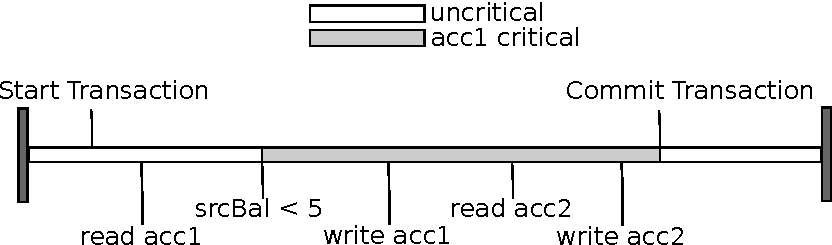
\includegraphics{Figures/lessCriticalValue}
\decoRule
\caption[Less Critical Value]{The critical time of the TVars in \code{limitedTransfer} with the alternative approach.}
\label{fig:lessCriticalValue}
\end{figure}
The TVar \code{acc2} is not critical at any point in the transaction because it is not needed for the control 
flow. \code{acc1} on the other hand becomes critical at the time its value is used to evaluate the branch
condition \code{(srcBal < am)}.

When the commit phase starts some reads are evaluated and some are unevaluated. Before the remaining
reads are evaluated the transaction acquires all locks for TVars it has modified. Chapter \ref{Chapter3} explains that it 
is enough to lock the TVars that are modfied instead of all TVars that were accessed. Then the transaction is validated.
This validation is similar to the validation in the original implementation; it is a comparision between
the values in the log (the TVars that the transaction needed to read to determine the control flow) and
the current values of these TVars. If all values match, the transaction is valid, otherwise it is invalid.
An invalid transaction is rolled back immediately after the locks are released. If the transaction is
valid, it finally executes the remaining \code{readTVar} operations in order to modify the 
actual TVars and determine the return value of the transaction. Then the modifications the transaction 
performed are committed to actual TVars. By committing the modifications the old values in the TVar are 
overwritten. This is the reason the \code{readTVar} operations can not be delayed any longer. 
Parallel to writing the actual TVars, the locks for these TVars are released. The last step of the transaction 
is to return the result. 

